% File project.tex
%% Style files for ACL 2021
\documentclass[11pt,a4paper]{article}
\usepackage[hyperref]{acl2021}
\usepackage{times}
\usepackage{booktabs}
\usepackage{todonotes}
\usepackage{latexsym}
\usepackage{multirow} 
\usepackage{xcolor}
\usepackage{graphicx}
\usepackage{hyperref}

\renewcommand{\UrlFont}{\ttfamily\small}

% This is not strictly necessary and may be commented out,
% but it will improve the layout of the manuscript,
% and will typically save some space.
\usepackage{microtype}

\aclfinalcopy 
% i\newcommand\BibTeX{B\textsc{ib}\TeX}

\title{11-777 Report 2: Baselines and Model Proposal}

\author{
  Ming-Feng Li\thanks{\hspace{4pt}Everyone Contributed Equally -- Alphabetical order} \hspace{2em} Pujith Kachana$^*$ \hspace{2em} Shashwat Chawla$^*$ \hspace{2em} Yatharth Ahuja $^*$ \\
  \texttt{\{mingfenl, pkachana, shashwac, yahuja\}@andrew.cmu.edu}
  }

\date{}

\begin{document}
\maketitle

\section{Baseline Models and Metrics (2 pages)}

We propose using a learning-based method that uses both LiDAR and RGB data for visual odometry. On that end, we believe that a natural progression of baselines would be unimodal classical approaches, unimodal learning-based approaches, multimodal classical approaches, and multimodal learning-based approaches. This set of baselines would help isolate the key distinguishing components of our proposed method and would serve as controlled comparisons for quantifying the benefits of learning-based approaches and multimodal approaches for visual odometry. These baselines will be evaluated on the KITTI dataset \cite{KITTI}, as it is the standard benchmark for visual odometry.

The first analysis we would like to perform is whether learning-based approaches can truly help achieve more accurate odometry. Given that odometry is geometrically grounded, it is possible to achieve high accuracies through classical optimization and heuristics alone. This can be seen in the case of works such as ICP-SLAM \cite{KISS-ICP} and ORB-SLAM \cite{orb-slam}, which are unimodal LiDAR and RGB models, respectively. These methods are still on the KITTI leaderboard, displaying the effectiveness of classical SLAM methods. Recent learning-based unimodal methods such as LO-Net \cite{lo-net} and TartanVO \cite{tartanvo} have shown competitive results as well, and we wish to study the effects of learning based methods in more detail.

The second analysis we aim to conduct focuses on the effects of fusing LiDAR and RGB data for odometry applications. Our investigation highlights the complementary strengths of these two modalities. RGB images provide rich, dense features that are useful for visual perception; however, they inherently lack 3D information, which can limit their effectiveness in spatial understanding. In contrast, LiDAR directly captures 3D points, but it often struggles to find correspondences between frames. We intend to explore the potential of these modalities to interact synergistically and mitigate each other's weaknesses. RGB can enhance the detail in areas where LiDAR data may be sparse or noisy, and LiDAR can improve spatial accuracy in regions where RGB images may struggle to find depth or features.

Previous works, particularly in classical LiDAR and RGB fusion techniques like V-LOAM \cite{vloam}, DV-LOAM \cite{dv-loam} and SDV-LOAM \cite{sdv-loam}, have demonstrated significant success in leveraging these modalities for odometry, as they are currently leading the KITTI leaderboard. Additionally, recent advancements in learning-based fusion methods such as DVLO \cite{dvlo} show promising potential for further improving performance. We intend to further explore multimodal learning-based approach, examining how the integration of LiDAR and RGB can lead to more robust and accurate visual odometry.\\

In the following section we explore the baselines which we use to explore and develop out proposed model.


% Please explain the baselines you are using. This includes (but is not limited to):
% \begin{enumerate}
%   \item Unimodal baselines
%   \item Very simple multimodal models  
%   \item Alternate choices for modules (e.g. encoders/decoders)
% \end{enumerate}

% (Explain all your choices and what types of interactions exist. What can a simple detector figure out of about the task? What can an LM infer from the prompt? What if I just pass detections to a model... -- you implement 2*N baselines -- these can use pretrained encoders/detectors)

\subsection{Unimodal Baselines}
\subsubsection{Classical}

\begin{table*}[t]
  \centering
  \caption{Comparison with different odometry networks on the KITTI odometry dataset. $t_{rel}$ and $r_{rel}$ mean the average sequence translational RMSE (\%) and the average sequence rotational RMSE ($^{\circ}$/100m) respectively on 06, 07, 09, 10 subsequences.\\ (*) Means learning based methods, whereas (-) means classical methods.} 

    \begin{tabular}{lllll|cc|cc|cc|cc}
    \toprule
    \multicolumn{5}{l|}{\multirow{2}[0]{*}{\textbf{Method}}} & \multicolumn{2}{c|}{06} & \multicolumn{2}{c|}{07} & \multicolumn{2}{c|}{09} & \multicolumn{2}{c}{10} \\
         &      &      &      &      & $t_{rel}$ & $r_{rel}$ & $t_{rel}$ & $r_{rel}$ & $t_{rel}$ & $r_{rel}$ & $t_{rel}$ & $r_{rel}$\\
    \midrule
    \multicolumn{13}{l}{\it{Visual Odometry Methods:}} \\
    \midrule
    \multicolumn{5}{l|}{ORB-SLAM (-)} & 18.68 & 0.26 & 10.96 & 0.37 & 15.3 & \textbf{0.26} & 3.71 & \textbf{0.3}  \\
    \multicolumn{5}{l|}{TartanVO (*)} & 4.72 & 2.95 & 4.32 & 3.41 & 6.0 & 3.11 & 6.89 & 2.73 \\
    \midrule
    \multicolumn{13}{l}{\it{LiDAR Odometry Methods:}} \\
    \midrule
    \multicolumn{5}{l|}{ICP-SLAM (-)} & 1.95 & 1.59 & 5.17 & 3.35 & 6.93 & 2.89 & 8.91 & 4.74  \\
    \multicolumn{5}{l|}{LO-Net (*)} & 1.04 & 0.69 & 0.71 & 0.50 & 2.12 & 0.77 & 1.80 & 0.93 \\
    \midrule
    \multicolumn{13}{l}{\it{Multimodal Odometry Methods:}} \\
    \midrule
    \multicolumn{5}{l|}{H-VLO (*)} & 0.75 & 0.30 & 0.79 & 0.48 & 1.89 & 0.34 & 1.36 & 0.43 \\
    \multicolumn{5}{l|}{DVLO (*)} & \textbf{0.33} & \textbf{0.17} & \textbf{0.46} & \textbf{0.33} & 0.85 & 0.36 & 0.88 & 0.46 \\
    \multicolumn{5}{l|}{DV-LOAM (-)} & 0.65 & 0.33 & 0.51 & \textbf{0.33} & 0.73 & 0.32 & 0.87 & 0.38 \\
    \multicolumn{5}{l|}{SDV-LOAM (-)} & 0.50 & 0.27 & 0.84 & 0.53 & \textbf{0.63} & 0.34 & \textbf{0.68} & 0.41 \\
    % \midrule
    
    \bottomrule
    \end{tabular}%
  \label{tab:evaluation_06_10}%
\end{table*}


For the RGB modality, we will use the classical unimodal baseline \textbf{ORB-SLAM} \cite{orb-slam}. This method extracts ORB features from images and uses them to establish correspondences between consecutive frames. By applying epipolar constraints and classical optimization techniques, it estimates camera poses, which are further refined through global optimization using a pose graph and loop closure. ORB-SLAM will establish a baseline for the accuracy achievable with monocular RGB images and geometric analysis, supporting our hypothesis that RGB images provide strong visual features for odometry.

For the LiDAR modality, we will use \textbf{ICP-SLAM} \cite{KISS-ICP} as an unimodal classical baseline. ICP (Iterative Closest Points) computes correspondences between two point sets by identifying the nearest neighbors and then calculating the transformation that minimizes the distance between these approximated correspondences. This process is repeated until the transformation converges below a threshold or reaches a maximum number of iterations. ICP can be effective with consecutive frames, although its accuracy diminishes in the presence of noise or lower sampling rates. This method will serve as a baseline to gauge the accuracy achievable with LiDAR alone and assess how well LiDAR’s inherent 3D structure can be utilized.

\subsubsection{Learning-Based}

\textbf{TartanVO} \cite{tartanvo} will serve as our learning-based unimodal baseline using RGB images. As one of the top-performing odometry models for monocular images, TartanVO is trained exclusively on the TartanAir dataset \cite{tartanair}, which we will also employ. This baseline will demonstrate the advantages of large-scale data and learning-based approaches while validating the effectiveness of the TartanAir dataset.

\textbf{LO-Net} \cite{lo-net} will be our learning-based unimodal baseline using LiDAR data. It leverages a novel weighted geometric constraint loss to efficiently extract features from point clouds. This baseline will help establish a benchmark for widely deployed LiDAR-based odometry solutions across various datasets, including TartanAir.

\subsection{Multimodal Baselines}
\subsubsection{Classical}
For the multimodal baselines, we will use \textbf{DV-LOAM} \cite{dv-loam} and \textbf{SDV-LOAM} \cite{sdv-loam}, both of which integrate visual and LiDAR information to enhance the accuracy and robustness of odometry and mapping tasks. The former employs frame-to-frame tracking and sliding window optimization for efficient pose estimation, refining keyframe poses using LiDAR data, which is particularly advantageous in environments with sparse visual features. The latter builds upon this by incorporating semi-direct approaches, such as LiDAR-Assisted Visual Odometry, which improves depth estimation and supports dynamic environments. Additionally, its cascaded Vision-LiDAR architecture balances direct visual odometry with precise LiDAR measurements, providing more accurate and robust pose estimates.


\subsubsection{Learning-Based}
To establish learning-based multimodal baselines, we used \textbf{H-VLO} \cite{hvlo} and \textbf{DVLO} \cite{dvlo}.\\
\textbf{H-VLO} is a straightforward learning-based multimodal baseline that estimates relative camera poses by fusing RGB images with LiDAR data. It first densifies a LiDAR scan using a deep depth completion network, which is then fused with estimated depth maps and RGB values from the images. This approach intuitively constructs data representations that assist in pose prediction and odometry, emphasizing the importance of preprocessing and fusing sensor data into meaningful intermediate representations for improved pose estimation. \\
Recently, \textbf{DVLO} has addressed the limitations of simple RGB-LiDAR fusion, which often overlooks critical spatial information. DVLO applies global and local fusion techniques, resulting in significant performance improvements on benchmark datasets. We plan to incorporate these techniques into our own fusion and encoding approach.

\subsection{Competitive Baselines}
To assess performance and maintain diversity among our baselines, we evaluated a total of eight baselines. These included both unimodal (Lidar and Visual) and multimodal approaches, as well as classical and learning-based methods for each approach, as detailed in Table \ref{tab:evaluation_06_10}. Among these, the baseline that demonstrated one of the best performances on the KITTI odometry dataset for trajectories 06, 07, 09, and 10 was \textbf{DVLO}. This was determined based on the average translational RMSE (\%) and average rotational RMSE ($^{\circ}$/100m). However, since this paper is a recent development and the code was uploaded to GitHub just five days ago, there were issues when we attempted to run it. Therefore, the results reported for this baseline are sourced from their paper. 
For the unimodal baseline, the monocular learning-based \textbf{TartanVO} performed well. TartanVO has been recognized for its impressive real-time efficiency and generalizability across various datasets and real-world scenarios, outperforming many geometry-based methods in challenging environments even while being trained on just synthetic dataset TartanAir.

Some of the key insights from evaluating these baselines are as follows:
\begin{enumerate}
  \item \textbf{ORB-SLAM}:  This method exhibited relatively poor performance in featureless areas and dynamic environments. However, as shown in Table \ref{tab:evaluation_06_10}, ORB-SLAM performed well in terms of rotational error.
  \item \textbf{TartanVO}: This monocular, learning-based visual odometry method outperformed other similar methods. Its superior performance is attributed to a diverse training dataset and the incorporation of camera intrinsic parameters into its architecture.
  \item \textbf{DVLO}: It utilizes a local-to-global feature fusion approach, integrating features from both narrow receptive fields and broader global contexts. This strategy enhances its performance by effectively combining local details and global information from visual and LiDAR data.
\end{enumerate}

% \clearpage


% \begin{table}[t]
% \centering
% \begin{tabular}{@{}lrr@{}}
% \toprule
%                             & \multicolumn{2}{c}{Dev} \\
% Methods                     & Accuracy $\uparrow$ & $L_2$ Error $\downarrow$  \\
% \midrule
% ORB-SLAM \cite{orb-slam} & & \\
% TartanVO \cite{tartanvo} & & \\
% ?????\cite{} & & \\
% \midrule
% ICP-SLAM \cite{KISS-ICP} & & \\
% LO-NET \cite{lo-net} & & \\
% ?????\cite{} & & \\
% \midrule
% V-LOAM \cite{vloam} & & \\
% DVLO \cite{dvlo} & & \\
% ?????\cite{} & & \\
% \bottomrule
% \end{tabular}
% \end{table}


\section{Results (1 page)}
As reported in Table \ref{tab:evaluation_06_10}, the metrics we are considering for our use-case and application are \textit{$t_{rel}$} and \textit{$r_{rel}$}, which report the relative translation and rotational error, respectively. These metrics are elaborated as follows.

\paragraph{\textbf{Metric 1,   }\textit{$t_{rel}$}:}
This metric represents the average relative translation error in the trajectory across the sequence. It is computed as:
\[
t_{rel} = \frac{1}{N} \sum_{i=1}^{N} \frac{\|\mathbf{t}_i - \mathbf{t}_i^{gt}\|}{\|\mathbf{t}_i^{gt}\|}
\]
where $\mathbf{t}_i$ is the estimated translation for frame $i$, $\mathbf{t}_i^{gt}$ is the ground truth translation, and $N$ is the number of frames.

\paragraph{\textbf{Metric 2,   }\textit{$r_{rel}$}:}
This metric reports the average relative rotation error in the trajectory across the sequence. It is computed as:
\[
r_{rel} = \frac{1}{N} \sum_{i=1}^{N} \text{arccos} \left( \frac{\text{trace}(\mathbf{R}_i^{gt} \mathbf{R}_i^\top) - 1}{2} \right)
\]
where $\mathbf{R}_i$ is the estimated rotation matrix for frame $i$, $\mathbf{R}_i^{gt}$ is the ground truth rotation matrix, and $N$ is the number of frames. \\

As we can see in table \ref{tab:evaluation_06_10}, multimodal methods prove to be much better than unimodal models, as both RGB and LiDAR modalities have their inherent distinctions. However, monocular estimations work well for rotational estimations in the pose.

\begin{figure*} [t]
    \centering
    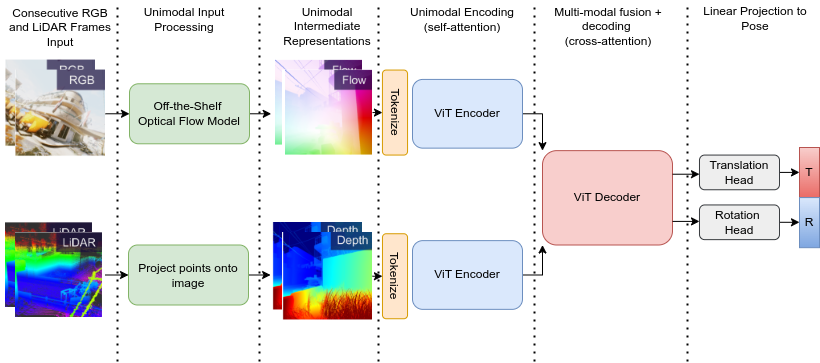
\includegraphics[width=0.95\linewidth]{Reports/2-Baselines-and-Model-Proposal/images/vol_model.png}
    \caption {The VOL model diagram. Given RGB and LiDAR frames from two consecutive timesteps, the model computes optical flow and aligns the LiDAR points to the point map. These intermediate representations are then processed by the separate encoder and combined into a decoder, and lastly sent through translation and rotation heads to recover pose.}
    \label{fig:model-diagram}
\end{figure*}



\section{Model Proposal}

\subsection{Overall model structure}
The model first consists of a preprocessing step for both the RGB images and LiDAR point clouds. The images are sent through an optical flow regression model to get an intermediary flow representation, and the point clouds are projected onto the image to enforce explicit matching between the 2D pixels and the corresponding 3D points. These processed modalities will then be sent through their respective ViT encoders and then combined with a ViT decoder and a projection head to output pose. In figure \ref{fig:tartanvo-opticalflow}, the bottom image, illustrates the optical flow representation while executing the TartanVO baseline on KITTI Odometry Trajectory - Sequence 10. This visualization provided valuable insights that informed the design of the model's structure. 

\begin{figure}[t]
    \centering
    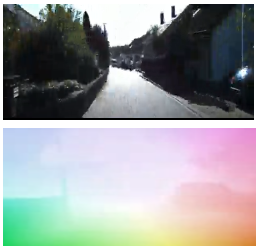
\includegraphics[width=1.0\linewidth]{Reports/2-Baselines-and-Model-Proposal/images/kitti10--inp_flow_10sec.png}
    \caption{The top image displays the model input from the left image of KITTI Odometry Trajectory 10 at 10 seconds, while the bottom image shows the corresponding optical flow output.}
    \label{fig:tartanvo-opticalflow}
\end{figure}
% \clearpage

\subsection{Encoders}
\subsubsection{RGB}
For the image encoder, we are considering two possibilities: a convolution (CNN) encoder \cite{cnn}, such as a ResNet backbone \cite{resnet}, for a Vision Transformer (ViT) encoder \cite{vit}. The CNN encoder would be efficient and simple, as there are already several effective pre-trained CNN backbones. However, its receptive field may be an issue. A ViT encoder will require more memory and computation, as it will need to perform self-attention over CNN patches, but it will have a more global understanding of the images. We are currently planning on using a ViT encoder for this global understanding and for downstream cross-attention with the patches.

\subsubsection{LiDAR}
For the LiDAR encoder, the naive approach would be to just voxelize the point cloud and use 3D convolutions as an encoder. However, this will be very inefficient, as 3D voxels are quite sparse and the receptive field issue will be exacerbated. An alternate approach is to use a point cloud-specific encoder such as PointNet \cite{pointnet} to induce useful properties such as permutation invariance. Lastly, we can preprocess the point cloud by projecting it onto the image space, such that the 3D points are in the shape of the image but contain $(x,y,z)$ values instead of $(R, G, B)$ as shown in DVLO \cite{dvlo}. This "point-map" 3D representation has been shown to be very effective in relating 2D RGB images to 3D points, as seen in works like DUSt3R \cite{dust3r}. We can then use the same encoder as used for the RGB images on these point maps, thus making the shared space between the two modalities more homogeneous.

\subsection{Decoders}
The decoder will be a ViT decoder architecture that performs cross-attention between the intermediate flow and pointmap encodings. This mechanism will allow for effective global information sharing between the two modalities. The output of this module will then be sent to separate heads for rotation and translation similar to the TartanVO architecture \cite{tartanvo}, enabling precise recovery of pose parameters. An alternate decoding scheme could be to concatenate the intermediate representations along the channel dimension and use a convolutional decoder to regress the pose. This approach will be more efficient, but will not have the rich, global information-sharing capabilities of the cross-attention and will suffer from its receptive field.

\subsection{Loss Functions}
% Describe both your primary task loss and three possible auxiliary losses that might improve performance.  Justify your choices.

The primary objective used to train the model will be a simple mean-squared error on the predicted translation and rotation.

\begin{equation} \label{eq:sim1}
L_{pose} = \|\hat{T} - T\| + \|\hat{R} - R\|
\end{equation}

This is based on the objective used for TartanVO \cite{tartanvo}, but uses absolute translation error instead of up-to-scale error since we wish to determine absolute pose. 

Some auxiliary losses that we believe would greatly help in inducing relevant biases for the model are optical flow and depth prediction for the RGB images. 

\begin{equation}
    L_{flow} = \sum_{i=1}^{N}||\mathbf{f}_{gt} - \mathbf{f}_i||_1
\end{equation}

\begin{equation}
    L_{depth} = \sum_{i=1}^{N}||\mathbf{d}_{gt} - \mathbf{d}_i||_2
\end{equation}


The flow loss will help the model learn explicit correspondences between two RGB frames. This essentially means that the model will learn where points have moved in 2D. Coupled with depth information, the model can learn how the points move in 3D. This can help better align the 2D information with the 3D LiDAR data and can help simulate 3D flow. If accurate correspondences and 3D positions are given, then the pose can be simply estimated through classical techniques such as Orthogonal Procrustes alone. We expect that when equipped with these capabilities, learning-based methods will learn robust odometry estimation. This can just be a per-pixel binary cross entropy over a ground-truth semantically segmented image, where certain classes are labeled as distractors.

Lastly, an additional alternate loss we could consider could be detection loss. We could train the model to also detect the pixels for key distractor objects, such as dynamic objects, potholes, etc such that the model will be able to ignore these in its odometry prediction.

\begin{equation}
L_{detection} = - \sum_{i=1}^{N} \left( y_i \log(\hat{y}_i) + (1 - y_i) \log(1 - \hat{y}_i) \right)
\end{equation}

In combination, the loss will look as follows:

\begin{equation}
    L_{total} = L_{pose} + \lambda_1*L_{flow} + \lambda_2*L_{depth} + \lambda_3*L_{detection}
\end{equation}

We hypothesize that the composition of these relevant auxiliary tasks will induce a robust and accurate objective for odometry.



% \clearpage
\section{Team member contributions}
\paragraph{Pujith} contributed baseline models introduction, ICP-SLAM, LOAM, V-LOAM, and LO-NET baselines, and model proposal.

\paragraph{Shashwat} contributed to the multimodal baseline models DV-LOAM, SDV-LOAM, TartanVO, the table for baseline comparison, the baseline comparison section, and the model proposal.

\paragraph{Yatharth Ahuja} contributed to the lidar based modality (LO-Net), monocular baseline (DPVO), multimodal baselines (H-VLO and DVLO), their results and comparisons, model proposal refinement, and report formatting. 

\paragraph{Ming-Feng Li} contributed to the table for baseline comparisons, evaluation metrics, and learning-based baseline model introduction.


% Please use 
\bibliographystyle{acl_natbib}
\bibliography{references}

%\appendix



\end{document}
